% !TeX program = uplatex
\documentclass[a4paper,12pt]{jlreq}

% ===== Packages =====
\usepackage{amsmath,amssymb,mathtools,bm}
\usepackage{siunitx}
\sisetup{detect-all,per-mode=symbol}
\usepackage{physics}
\usepackage{mhchem}
\usepackage{booktabs}
\usepackage{graphicx}
\usepackage{hyperref}
\usepackage{ascmac} % ← itembox 使うため
\usepackage{xcolor}
\usepackage{tikz}


\hypersetup{
  colorlinks=true,
  linkcolor=black,
  urlcolor=blue,
  citecolor=black
}

\usepackage{enumitem}
\usepackage{geometry}
\usepackage{fancybox}
\geometry{margin=25mm}

\title{入門電磁気学　レポート課題}
\author{学籍番号：2225091　西亦 岳雄}

\begin{document}
\maketitle



\begin{itembox}[l]{問}
　無限に長い一様なソレノイドコイル(半径$a$, 巻き数は単位長さあたり$n$とする)
の内部に, 中心軸と平行に2枚の平行平板を入れて, 
それぞれに$V_0, -V_0$の平板の電位をかけた.\par

　平行平板間のおける電子の運動を考察せよ.

\end{itembox}

\fbox{解答}\par




\section*{ソレノイドコイルに平行平板を入れたときの電子の運動}

半径$a$，単位長さあたりの巻き数$n$の無限に長い一様なソレノイドコイルに電流$I$を流すと，コイル内部にはz軸方向(上向き)にほぼ一様な磁場
\[
  \bm{B} = B\,\bm{e}_z, 　\bm{B} = \mu_0 n I \bm{e}_z
\]
が生じる。

\begin{figure}[hbtp]
  \centering
  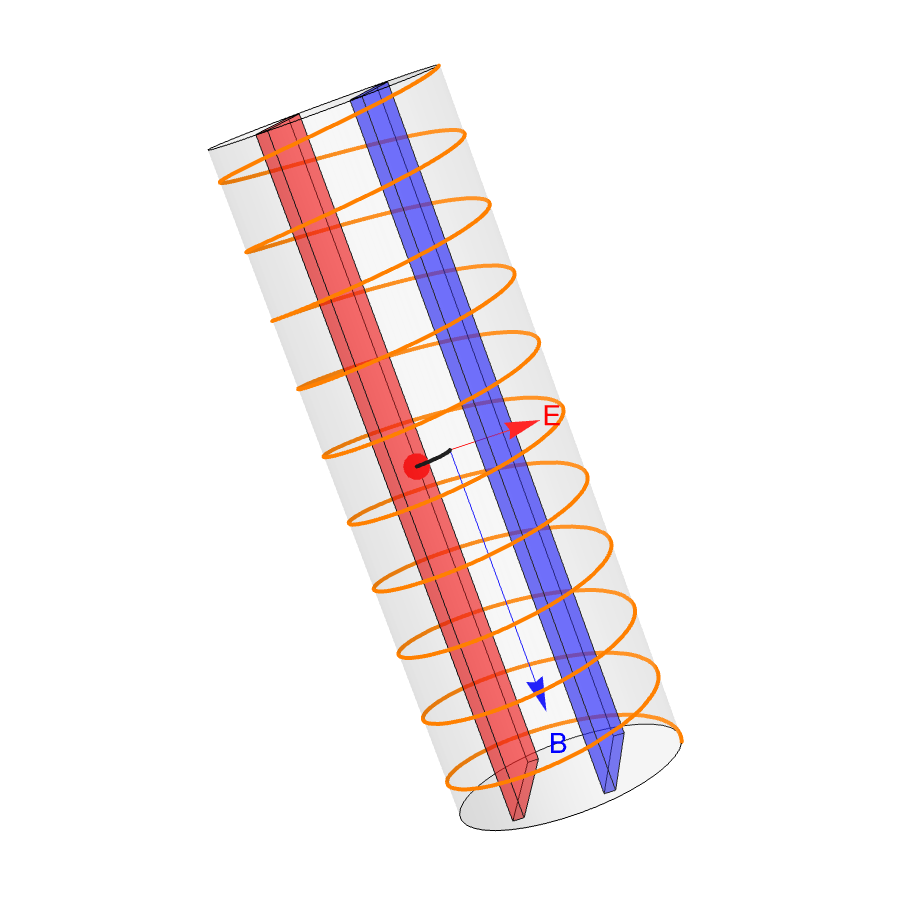
\includegraphics[width=0.6\linewidth]{images/electro_coil.png}
\end{figure}


ここで, ソレノイド内部に$z$軸と平行な2枚の平行平板を入れて,
軸から各平板までの距離を$d$とする。
一方の平板を電位$+V_0$，他方を電位$-V_0$をかけると, 
2枚の平板間の距離は $2d$，電位差は $2V_0$ であるから，
平板間には$z$軸に垂直で一様な電場
\[
  E = \frac{2V_0}{2d} = \frac{V_0}{d}
\]
が生じる. ここで,$E = -\frac{d\phi}{dx}$の関係を用いた. $x=-d$の板が $+V_0$, $x=+d$の板が$-V_0$のとき,
電場の向きは
\[
  \bm{E} = E\,\bm{e}_x
\]
と書ける.\par


\vspace{10mm}


電荷$-e$をもつ電子に働くローレンツ力は
\[
  \bm{F} = -e\bigl(\bm{E} + \bm{v}\times\bm{B}\bigr)
\]
である. 上記から
\[
  \bm{E} = E\,\bm{e}_x, \qquad \bm{B} = B\,\bm{e}_z
\]
であるから，電子の運動方程式は
\begin{align*} 
  m\dot v_x &= -e\bigl(E + v_y B\bigr), \\
  m\dot v_y &= e\,v_x B, \\
  m\dot v_z &= 0
\end{align*}
とかける。したがって電子は$x-y$平面のみで運動をする. \par



電場のみが電子に対して力を及ぼすとき, 
$m\dot v_x = -eE$，$m\dot v_y=0$ となり，
電子は$x$軸方向の電場の向きと反対，つまり$+V_0$ 側に向かって運動する。\par

磁場のみが電子に対して力を及ぼすとき, 
$m\dot{\bm v}=-e\,\bm{v}\times\bm{B}$ であり，
等速度で$\bm{B}$に垂直な平面上で円運動をする。
$v_z\neq 0$ なら軸方向に進みながららせん運動となる。


電子が電場と磁場両方から力を受けるとき, 上記の電子の運動方程式は
微分方程式であって, 

\[
\begin{aligned}
  \dot{v}_x &= -\frac{eB}{m} \left(v_y(t) - \frac{E}{B}\right) \\
  \dot{v}_y &= \frac{eB}{m} v_x(t)\\
  \dot{v}_z &= 0
\end{aligned}
\]
を解けば, 電子の動きがわかる. 
初期条件として, $v_x(0) = v_y(0) = v_z(0) = 0$, 
$x(0) = y(0) = z(0) = 0$と設定する. これを解くと

\[
\begin{aligned}
  x(t) &= \frac{E}{eB} (1 - \cos \omega t)\\
  y(t) &= \frac{E}{eB} (\omega t - \sin \omega t)
\end{aligned}
\]
となる. つまり, 電子は電場の影響により$x$軸の正方向に加速され, 
このとき, 電子は磁場の影響で回転していく. その後, 電子の運動方向は
$x$軸の負方向へと変化して, 電子は電場によって減速する. 

ここで
\[
  \omega = \frac{eB}{m}.
\]


すなわち電子は，$x$–$y$ 平面内で円運動をしながら，
その円の中心が $y$ 軸負方向へ一定速度 $E/B$ で力を受け, 
円運動でサイクロイドの軌道を描く。






\vspace{30mm}



電場が及ぼす力は
\[
  \bm{F}_E = -e\bm{E} = -eE\,\bm{e}_x
\]
であり，電場の向きと反対，つまり電位$+V_0$の平板へ電子を引き寄せる.
一方，磁場が及ぼすローレンツ力である
\[
  \bm{F}_B = -e\,\bm{v}\times\bm{B}
\]
は電子の速度ベクトル$\bm{v}$と常に直交しているため
\[
  \bm{v}\cdot\bm{F}_B = 0
\]
であるから，電子の運動エネルギーには寄与せず，
運動の方向のみに寄与する.
平行平板の電位が$+V_0$と$-V_0$で，
電子が$-V_0$の平板から$+V_0$の平板へ移るとき，
電位差は$2V_0$であるから，ポテンシャルエネルギーは
$\Delta U = q\Delta\phi = (-e)\cdot 2V_0 = -2eV_0$ だけ減少し，
運動エネルギーは
\[
  \Delta K = -\Delta U = 2eV_0
\]
だけ増加し, 磁場はエネルギーのやりとりには寄与しない.


\begin{itembox}[l]{概括}
ソレノイドコイル内部には軸方向の一様な磁場$\bm{B}$が生じていて, 
その内部に平行平板を置くと$z$軸に垂直で一様な電場$\bm{E}$が生じる.
電子は電場によって$+V_0$の平板へ加速される一方，
磁場によるローレンツ力によって軌道が曲げられ，
円運動をする.
その結果，電子は円運動と電場と磁場が直交しているために
生じる横方向の一様運動が重なった
サイクロイド（あるいは$v_z\neq 0$なららせん状）の軌道を描き，
最終的には$+V_0$の平板に衝突する。
電子の運動エネルギーを増やすのは電場だけであり，
磁場は運動の向きを変えるだけで仕事はしない。

\end{itembox}





\end{document}